\documentclass{article}
\usepackage[utf8]{inputenc}
\usepackage[UKenglish]{babel}
%\renewcommand{\familydefault}{\sfdefault}
\usepackage{ifpdf}
\usepackage{hyperref}
\usepackage{graphicx}
\usepackage{caption}
\usepackage{xspace}
\usepackage{xcolor,soul}

\definecolor{light-gray}{gray}{0.850}

\newcommand{\hlc}[2][yellow]{\sethlcolor{#1}\hl{#2}}
\newcommand{\class}[1]{\xspace{\small\hlc[light-gray]{\texttt{#1}}}\xspace}
\newcommand{\struct}[1]{\xspace{\small\hlc[light-gray]{\textsl{#1}}}\xspace}

\renewcommand{\arraystretch}{1.5} % space between table rows

\title{Ceph Mon: a technical overview}
\author{Paolo VIOTTI}
\date{\today}
\ifpdf
\hypersetup{
    pdfauthor={Paolo VIOTTI},
    pdftitle={Ceph Mon: a technical overview},
}
\fi
\begin{document}

\maketitle

\begin{abstract}
Ceph is a free software storage platform designed to provide object, block and file storage 
using computer clusters running on commodity hardware. 
Ceph's main design goals include high scalability, fault tolerance and low maintenance requirements.
This document provides an in-depth technical overview of the design of Ceph Monitor, 
i.e. the Ceph component in charge of maintaining a map of the cluster along with authorization information.
\end{abstract}

\section{Ceph: an introduction}
Ceph \cite{ceph} is a free software storage platform that provides object, block and file storage 
using computer clusters running on commodity hardware. 
Since its origin as a research project around 2006, 
Ceph has undergone constant and substantial development,
thus gaining popularity which is reflected by an ever increasing adoption as storage backend in state-of-the-art
high-end computing systems \cite{ceph-openstack}.

As illustrated in Fig. \ref{fig:stack}, Ceph exposes to application clients multiple APIs: 
\begin{itemize}
	\item a POSIX-compatible distributed file system (\textbf{Ceph FS}), built as Linux kernel module or user-space FUSE client;
	\item a REST-based storage gateway (\textbf{RADOSGW}) compatible with OpenStack Swift and Amazon S3;
	\item a block storage device (\textbf{RDB}) suitable for virtualization platforms making use of kernel 
	virtualization technologies such as QEMU or KVM.
\end{itemize}

\begin{center}
	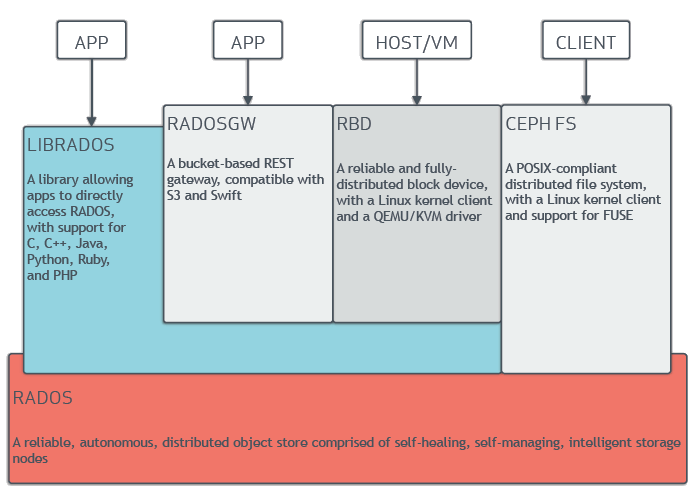
\includegraphics[scale=0.35]{figs/ceph-stack.png}
	\captionof{figure}{Ceph application stack}
	\label{fig:stack}
\end{center}

Beside, an application developer may even hook into the low level API exposed through \textbf{librados} 
and offered in several programming languages in order to directly connect with \textbf{RADOS} 
(\textit{Reliable Autonomic Distributed Object Store}), i.e. the inner object storage layer
that acts as foundation of the interfaces mentioned above.

The Ceph cluster consists of different components, running as distributed daemons:
\begin{itemize}
	\item Cluster monitors (\textit{ceph-mon}, or Mon) that keep track of active and failed cluster nodes;
	\item Metadata servers (\textit{ceph-mds}) that store the metadata of inodes and directories;
    \item Object storage devices (\textit{ceph-osd}) that actually store data on local filesystems;
    \item RESTful gateways (\textit{ceph-rgw}) that expose the object storage layer as an interface 
    compatible with Amazon S3 or OpenStack Swift APIs.
\end{itemize}

The rest of this document focuses on the monitor component, starting from its high-level architecture,
deep down to the implementation details present, to date, in its C++ codebase \cite{ceph-code}.
To marry the need for this 1000 ft. view with the requirement of presenting the related 
low level features, in the following sections informal functional descriptions may be presented beside
the name of their main corresponding entities in the code (e.g. \class{classes} or \struct{data structures}).
Most of the code required to run the monitor is contained in the \texttt{src/mon} directory of the repository  \cite{ceph-code}
($\sim$34k LOC), although it shares with the rest of the codebase few functions and classes related to
specific parts of the system (e.g. OSD or MDS daemons, respectively in \texttt{src/osd} and \texttt{src/mds}),
or networking, logging and other basic facilities.

\section{Ceph Mon}
A Ceph Monitor maintains a set of structured information about the cluster state, including:

\begin{itemize}
	\item the monitor map - \class{MonMap}
	\item the OSD map - \class{OSDMap}
	\item the Placement Group (PG) map - \class{PGMap}
	\item the MDS map - \class{MDSMap}.
\end{itemize}

Additionally, information about authorization and capabilities granted to users over the 
different components of the system is maintained. 
Besides, Ceph holds a history, as a sequence of \textit{epochs}, of each state change in the maps.
All these information are replicated across the ceph-mon instances - 
which are, for example, 3 or 5, deployed on different machines.
Each monitor replica keeps its data strongly consistent using an implementation of the 
Paxos consensus algorithm (\class{Paxos}).

\subsection{Architecture}

As illustrated in Fig. \ref{fig:monarch}, the Ceph monitor is composed by several sub-monitors which 
oversee different aspects of the cluster.
All these monitors refer to a unique instance of Paxos\footnote{This was not true before v0.58,
see: \url{http://ceph.com/dev-notes/cephs-new-monitor-changes/}}
in order to establish a total order between possibly concurrent operations and achieve strong consistency.
Thus, Paxos is agnostic of any semantic associated with the updates it helps ordering, as in fact
it just delivers blobs (i.e. \struct{bufferlist} as payload of \class{Message}).

\begin{center}
	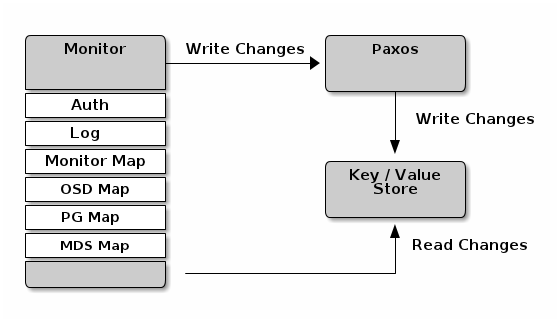
\includegraphics[scale=0.50]{figs/ceph-mon-arch.png}
	\captionof{figure}{Ceph Monitor high-level architecture}
	\label{fig:monarch}
\end{center}

\subsection{Code}

Table \ref{tab:class} shows an incomplete list of classes involved in the functioning of the monitor.
To each class is

\begin{center}
	\begin{tabular}{l|p{6cm}|p{5cm}}
		Entity & Purpose & Data and attributes \\ \hline
		\texttt{ceph\_mon.cc} & main entry point for monitor daemon and batch commands & - \\
		\class{Monitor} & 
		
		the main Monitor class 
		\begin{itemize}
		\item holds and start \class{Paxos}, 
		                 \class{MonitorDB}, \class{Messenger} and all the sub-monitors
		                 (\class{*Monitor}) 
        \item dispatch messages coming from \class{Messenger} to the sub-monitors 
        \end{itemize}		                 
		                 
		                 & 
		                \class{MonMap}, \class{KeyServer}, \class{KeyRing}, \class{Paxos},
		                \class{MonitorDBStore}\\
		%${41} & ${42} & ${43} \\\\
		%${51} & ${52} & ${53} \\\\
		%${61} & ${62} & ${63} \\\\
		%${71} & ${72} & ${73} \\\\
		%${81} & ${82} & ${83} \\\\
		%${91} & ${92} & ${93} \\\\
		%${101} & ${102} & ${103} \\\\
	\end{tabular}
	\captionof{table}{Main classes used by Ceph Monitor}
	\label{tab:class}
\end{center}

%During runtime operations, Ceph OSD Daemons check up on other Ceph OSD Daemons and report their findings to the Ceph Monitor.

monitor states



\begin{itemize}

\item \textit{probing}:
\item \textit{synchronizing}:
\item \textit{electing}:
\item \textit{leader}:
\item \textit{peon}:
\item \textit{shutdown}:




\begin{center}
	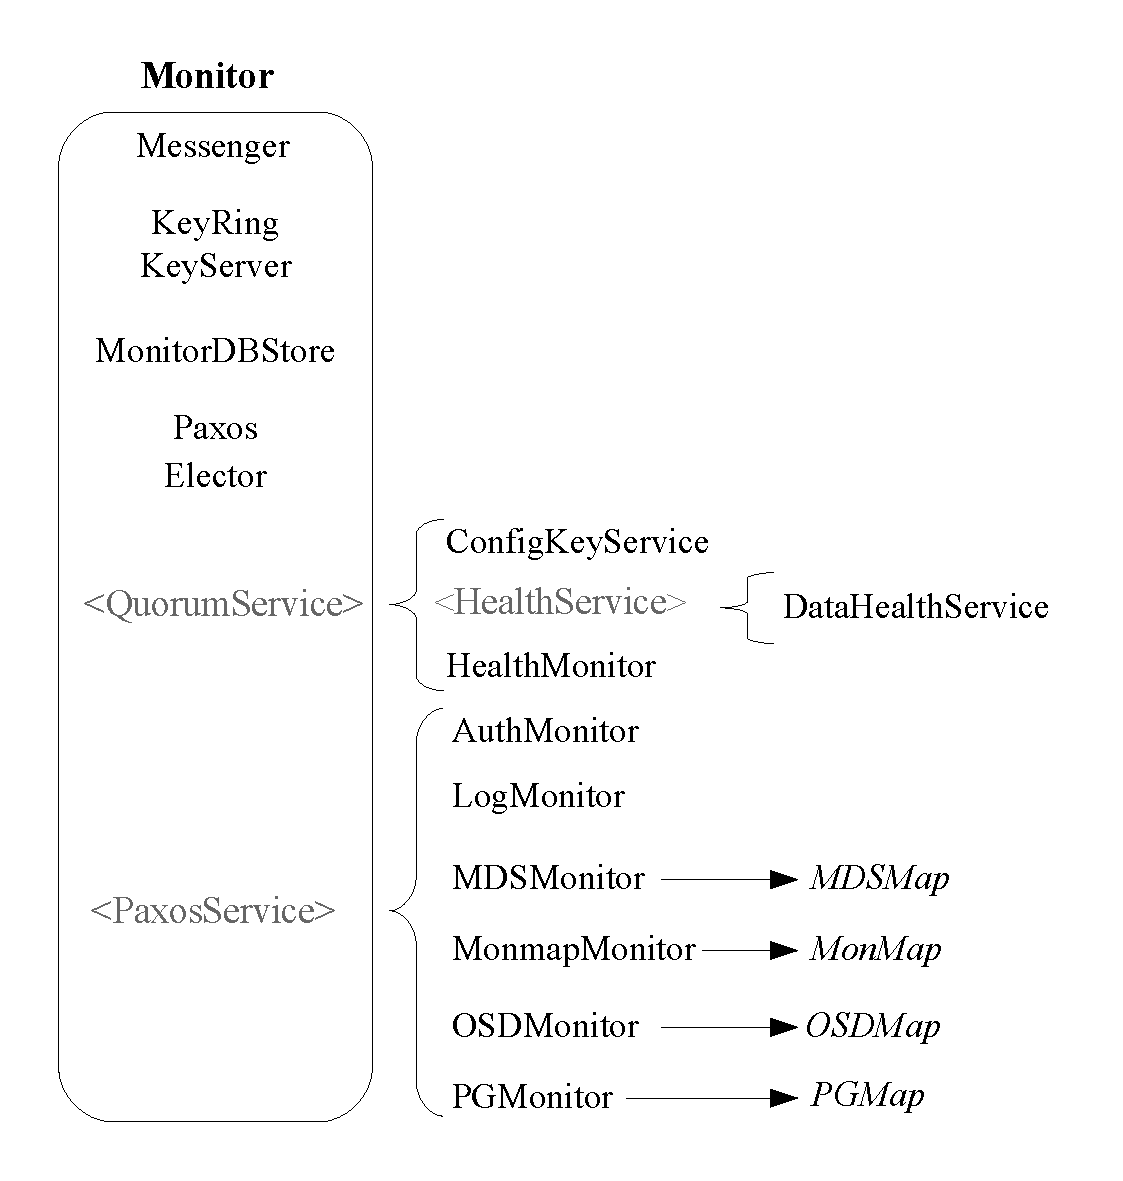
\includegraphics[scale=0.50]{figs/class_dia.pdf}
	\captionof{figure}{Ceph Monitor classes}
	\label{fig:monclass}
\end{center}


\subsection{Paxos}

Paxos states:


Paxos transitions


\subsection{Additional notes}

\begin{verbatim}
To ask / understand:
 
 - MonitorStore.{h,cc} never used
 - difference between MonCommands and DumplingMonCommands?


\end{verbatim}


\begin{thebibliography}{1}

  \bibitem{ceph} Ceph storage platform. \url{http://ceph.com/} 

  \bibitem{ceph-openstack} OpenStack User Survey Insights: November 2014. \\
  \url{http://perma.cc/367D-G5YN} 
  
  \bibitem{ceph-code} Ceph source code. \url{https://github.com/ceph/ceph} 

  %\bibitem{fo} Bob Tadashi Wakabayashi {\em Anti-Foreignism and Western
  %Learning in Early-Modern Japan} 1986: Harvard University Press.

\end{thebibliography}
	
\end{document}
